% $Header: /cvsroot/latex-beamer/latex-beamer/solutions/generic-talks/generic-ornate-15min-45min.en.tex,v 1.4 2004/10/07 20:53:08 tantau Exp $

\documentclass[svgnames]{beamer}

% This file is a solution template for:

% - Giving a talk on some subject.
% - The talk is between 15min and 45min long.
% - Style is ornate.

% Copyright 2004 by Till Tantau <tantau@users.sourceforge.net>.
%
% In principle, this file can be redistributed and/or modified under
% the terms of the GNU Public License, version 2.
%
% However, this file is supposed to be a template to be modified
% for your own needs. For this reason, if you use this file as a
% template and not specifically distribute it as part of a another
% package/program, I grant the extra permission to freely copy and
% modify this file as you see fit and even to delete this copyright
% notice. 

\newcommand\independent{\protect\mathpalette{\protect\independenT}{\perp}}
\def\independenT#1#2{\mathrel{\rlap{$#1#2$}\mkern2mu{#1#2}}}

\mode<presentation>
{
  \usetheme{Singapore}
  % or ...

  \setbeamercovered{transparent}
  % or whatever (possibly just delete it)
}

\usepackage{tikz}
\usepackage{pgflibraryarrows}

\usepackage{babel}
% or whatever

\usepackage[latin1]{inputenc}
% or whatever

\usepackage{upquote}

%\usepackage{times}
%\usepackage[T1]{fontenc}
% Or whatever. Note that the encoding and the font should match. If T1
% does not look nice, try deleting the line with the fontenc.


\title[R history] % (optional, use only with long paper titles)
{History and Ecology of R}

\subtitle
{} % (optional)

\author % (optional, use only with lots of authors)
{Martyn Plummer}
% - Use the \inst{?} command only if the authors have different
%   affiliation.

\institute[IARC] % (optional, but mostly needed)
{
  University of Warwick, UK
}
% - Use the \inst command only if there are several affiliations.
% - Keep it simple, no one is interested in your street address.

\date % (optional)
{SPE 2019, Tartu}

\subject{Talks}
% This is only inserted into the PDF information catalog. Can be left
% out. 

% If you have a file called "university-logo-filename.xxx", where xxx
% is a graphic format that can be processed by latex or pdflatex,
% resp., then you can add a logo as follows:

% \pgfdeclareimage[height=0.5cm]{university-logo}{university-logo-filename}
% \logo{\pgfuseimage{university-logo}}

% If you wish to uncover everything in a step-wise fashion, uncomment
% the following command: 

%\beamerdefaultoverlayspecification{<+->}

%Include IARC logo as background in slides
%\setbeamertemplate{background canvas}{\includegraphics
%        [width=\paperwidth,height=\paperheight]{figures/logobg.jpg}}

\begin{document}

%{%Temporarily reset background for front page
%\setbeamertemplate{background canvas}{\includegraphics
%        [width=\paperwidth,height=\paperheight]{figures/iarcbg.jpg}}
\begin{frame}[plain]
  \titlepage
\end{frame}
%}

% Since this a solution template for a generic talk, very little can
% be said about how it should be structured. However, the talk length
% of between 15min and 45min and the theme suggest that you stick to
% the following rules:  

% - Exactly two or three sections (other than the summary).
% - At *most* three subsections per section.
% - Talk about 30s to 2min per frame. So there should be between about
%   15 and 30 frames, all told.

%\AtBeginSection[]
%{
%  \begin{frame}<beamer>
%    \frametitle{Outline}
%    \tableofcontents[currentsection,currentsubsection]
%  \end{frame}
%}

%\AtBeginSubsection[]
%{
%  \begin{frame}<beamer>
%    \frametitle{Outline}
%    \tableofcontents[currentsection,currentsubsection]
%  \end{frame}
%}

\section{Pre-history}

\begin{frame}
  \frametitle{Pre-history}

  \begin{center}
  {\em Before there was R, there was S.}
  \end{center}
  
\end{frame}

\begin{frame}
  \frametitle{The S language}

  Developed at AT\&T Bell laboratories by Rick Becker, John Chambers,
  Doug Dunn, Paul Tukey, Graham Wilkinson.

  ~\\
  
  {\small
    \begin{tabular}{|lll|}
      \hline
      Version 1 & 1976--1980 & Honeywell GCOS, Fortran-based \\
      \hline
      Version 2 & 1980--1988 & Unix; Macros, Interface Language \\
      & 1981--1986 & QPE {\tiny (Quantitative  Programming Environment)} \\
      & 1984--     & General outside licensing; books \\
      \hline
      Version 3 & 1988-1998 & C-based; S functions and objects \\
      & 1991-- & Statistical models; \\
      &        & informal classes and methods \\
      \hline
      Version 4 & 1998 & Formal class-method model; \\
      & & connections; large objects\\
      & 1991-- & Interfaces to Java, Corba?\\
      \hline
    \end{tabular}
  }
  
  {\tiny Source: Stages in the Evolution of S
    \url{http://ect.bell-labs.com/sl/S/history.html}}

\end{frame}

\begin{frame}
  \frametitle{The ``Blue Book'' and the ``White Book''}

  \begin{columns}
    \begin{column}{2cm}
      \resizebox{2cm}{!}{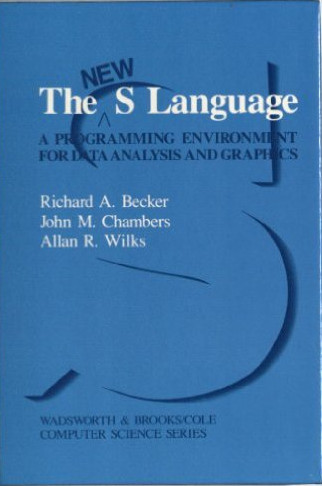
\includegraphics{figures/blue_book.jpg}}
      \resizebox{2cm}{!}{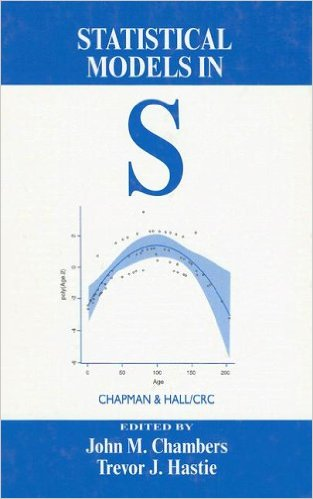
\includegraphics{figures/white_book.jpg}}
    \end{column}
    \begin{column}{8cm}
      Key features of S version 3 outlined in two books:
      \begin{itemize}
        \item Becker, Chambers and Wilks, {\em The New S Language: A
          Programming Environment for Statistical Analysis and
          Graphics} (1988)
          \begin{itemize}
          \item Functions and objects
          \end{itemize}
        \item Chambers and Hastie (Eds), {\em Statistical Models in S} (1992)
          \begin{itemize}
          \item Data frames, formulae
          \end{itemize}
      \end{itemize}
      These books were later used as a prototype for R.
    \end{column}
  \end{columns}

\end{frame}

\begin{frame}
  \frametitle{Programming with Data}

  \begin{quote}
  ``We wanted users to be able to begin in an interactive environment,
  where they did not consciously think of themselves as programming. Then
  as their needs became clearer and their sophistication increased, they
  should be able to slide gradually into programming.''
  -- John Chambers, Stages in the Evolution of S
  \end{quote}

  This philosophy was later articulated explicitly in {\em Programming
    With Data} (Chambers, 1998) as a kind of mission statement for S

  \begin{quote}
    To turn ideas into software, quickly and faithfully
  \end{quote}
  
\end{frame}

\begin{frame}
  \frametitle{The ``Green Book''}

  \begin{columns}
    \begin{column}{2.5cm}
      \resizebox{2.5cm}{!}{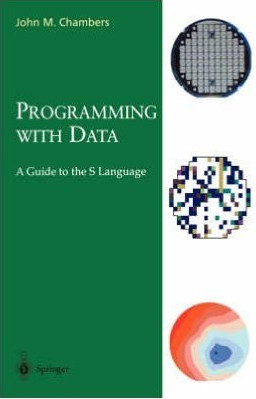
\includegraphics{figures/green_book.jpg}}
    \end{column}
    \begin{column}{7cm}
      Key features of S version 4 were outlined in Chambers, {\em Programming
      with Data} (1998).
      \begin{itemize}
      \item S as a programming language
      \item Introduced formal classes and methods, which were later
        introduced into R by John Chambers himself.
      \end{itemize}
    \end{column}
  \end{columns}

\end{frame}

\begin{frame}
  \frametitle{S-PLUS}

  \begin{itemize}
  \item AT\&T was a regulated monopoly with limited ability to exploit
    creations of Bell Labs.
  \item S source code was supplied for free to universities
  \item After the break up of AT\&T in 1984 it became possible for them
    to sell S.
  \item S-PLUS was a commercially available form of S licensed to
    Statistical Sciences (later Mathsoft, later Insightful) with added
    features:
    \begin{itemize}
    \item GUI,survival analysis, non-linear mixed effects, Trellis
      graphics, ...
    \end{itemize}
  \end{itemize}
  
\end{frame}

\begin{frame}
  \frametitle{The Rise and Fall of S-PLUS}
    
  \begin{itemize}
  \item 1988. Statistical Science releases first version of S-PLUS.
  \item 1993. Acquires exclusive license to distribute S. Merges with Mathsoft.
  \item 2001. Changes name to Insightful.
  \item 2004. Purchases S language for \$2 million.
  \item 2008. Insightful sold to TIBCO. S-PLUS incorporated into TIBCO Spotfire.
  \end{itemize}

\end{frame}

\section{History}

\begin{frame}
  \frametitle{History}

  \begin{center}
    {\em How R started, and how it turned into an S clone}
  \end{center}

\end{frame}

\begin{frame}
  \frametitle{The Dawn of R}

  \begin{columns}
    \begin{column}{2.5cm}
      \resizebox{2.5cm}{!}{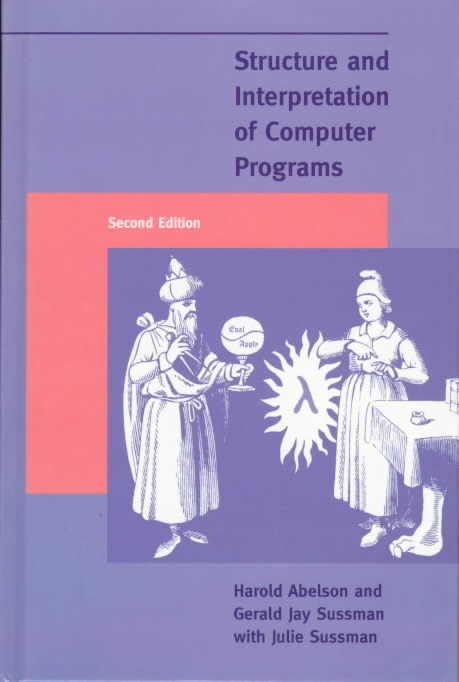
\includegraphics{figures/wizard_book.jpg}}
    \end{column}
    \begin{column}{7.5cm}
      \begin{itemize}
      \item Ross Ihaka and Robert Gentlemen at the University of Auckland
      \item An experimental statistical environment
      \item Scheme interpreter with S-like syntax
        \begin{itemize}
        \item Replaced scalar type with vector-based types of S
        \item Added lazy evaluation of function arguments
        \end{itemize}
      \item Announced to {\em s-news} mailing list in August 1993.
      \end{itemize}
    \end{column}
  \end{columns}

\end{frame}

\begin{frame}
  \frametitle{A free software project}

  \begin{itemize}
  \item June 1995. Martin Maechler (ETH, Zurich) persuades Ross and
    Robert to release R under GNU Public License (GPL)
  \item March 1996. Mailing list {\em r-testers} mailing list
    \begin{itemize}
    \item Later split into three {\em r-announce}, {\em r-help}, and
      {\em r-devel}.
    \end{itemize}
  \item Mid 1997. Creation of {\em core team} with access to central
    repository (CVS)
    \begin{itemize}
    \item {\small Doug Bates, Peter Dalgaard, Robert Gentleman, Kurt
      Hornik, Ross Ihaka, Friedrich Leisch, Thomas Lumley, Martin
      Maechler, Paul Murrell, Heiner Schwarte, Luke Tierney}
    \end{itemize}
  \item 1997. Adopted by the GNU Project as ``GNU S''. 
  \end{itemize}
\end{frame}
  
\begin{frame}
  \frametitle{The draw of S}

  \begin{quote}
    ``Early on, the decision was made to use S-like syntax. Once that
    decision was made, the move toward being more and more like S has
    been irresistible''\\
    -- Ross Ihaka, R: Past and Future History
    (Interface '98)
  \end{quote}

  R 1.0.0, a complete and stable implementation of S version 3, was
  released in 2000.

\end{frame}

\begin{frame}
  \frametitle{A Souvenir}

  \centering
  \resizebox{7cm}{!}{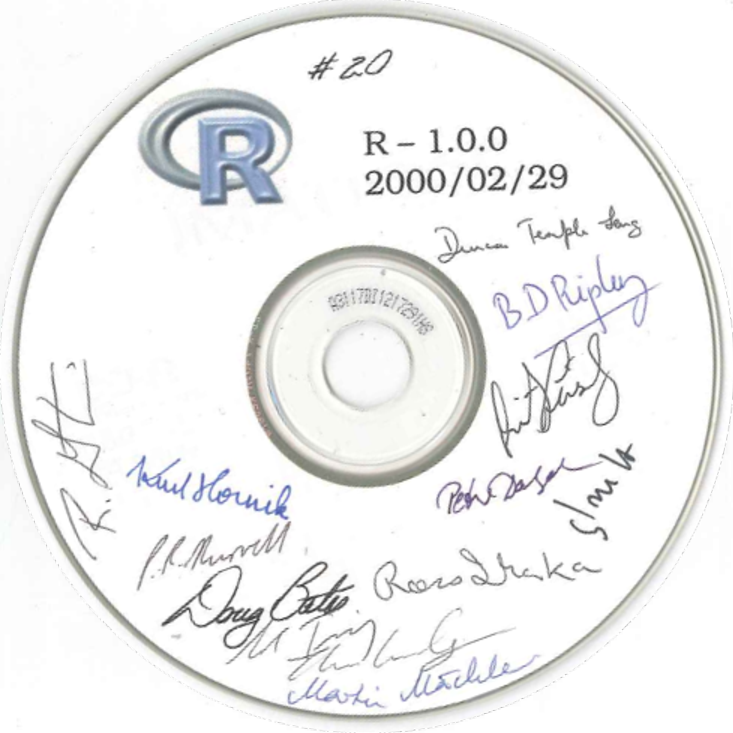
\includegraphics{figures/R-disk.pdf}}

\end{frame}

\begin{frame}
  \frametitle{Packages}

  \begin{itemize}
  \item Comprehensive R Archive Network (CRAN) started in 1997
    \begin{itemize}
    \item Quality assurance tools built into R
    \item Increasingly demanding with each new R release
    \end{itemize}
  \item Recommended packages distributed with R
    \begin{itemize}
    \item Third-party packages included with R distribution
    \item Provide more complete functionality for the R environment
    \item Starting with release 1.3.0 (completely integrated in 1.6.0)
    \end{itemize}
  \end{itemize}
  
\end{frame}

\begin{frame}
  \frametitle{Growth of CRAN}

  \begin{center}
  \resizebox{7cm}{!}{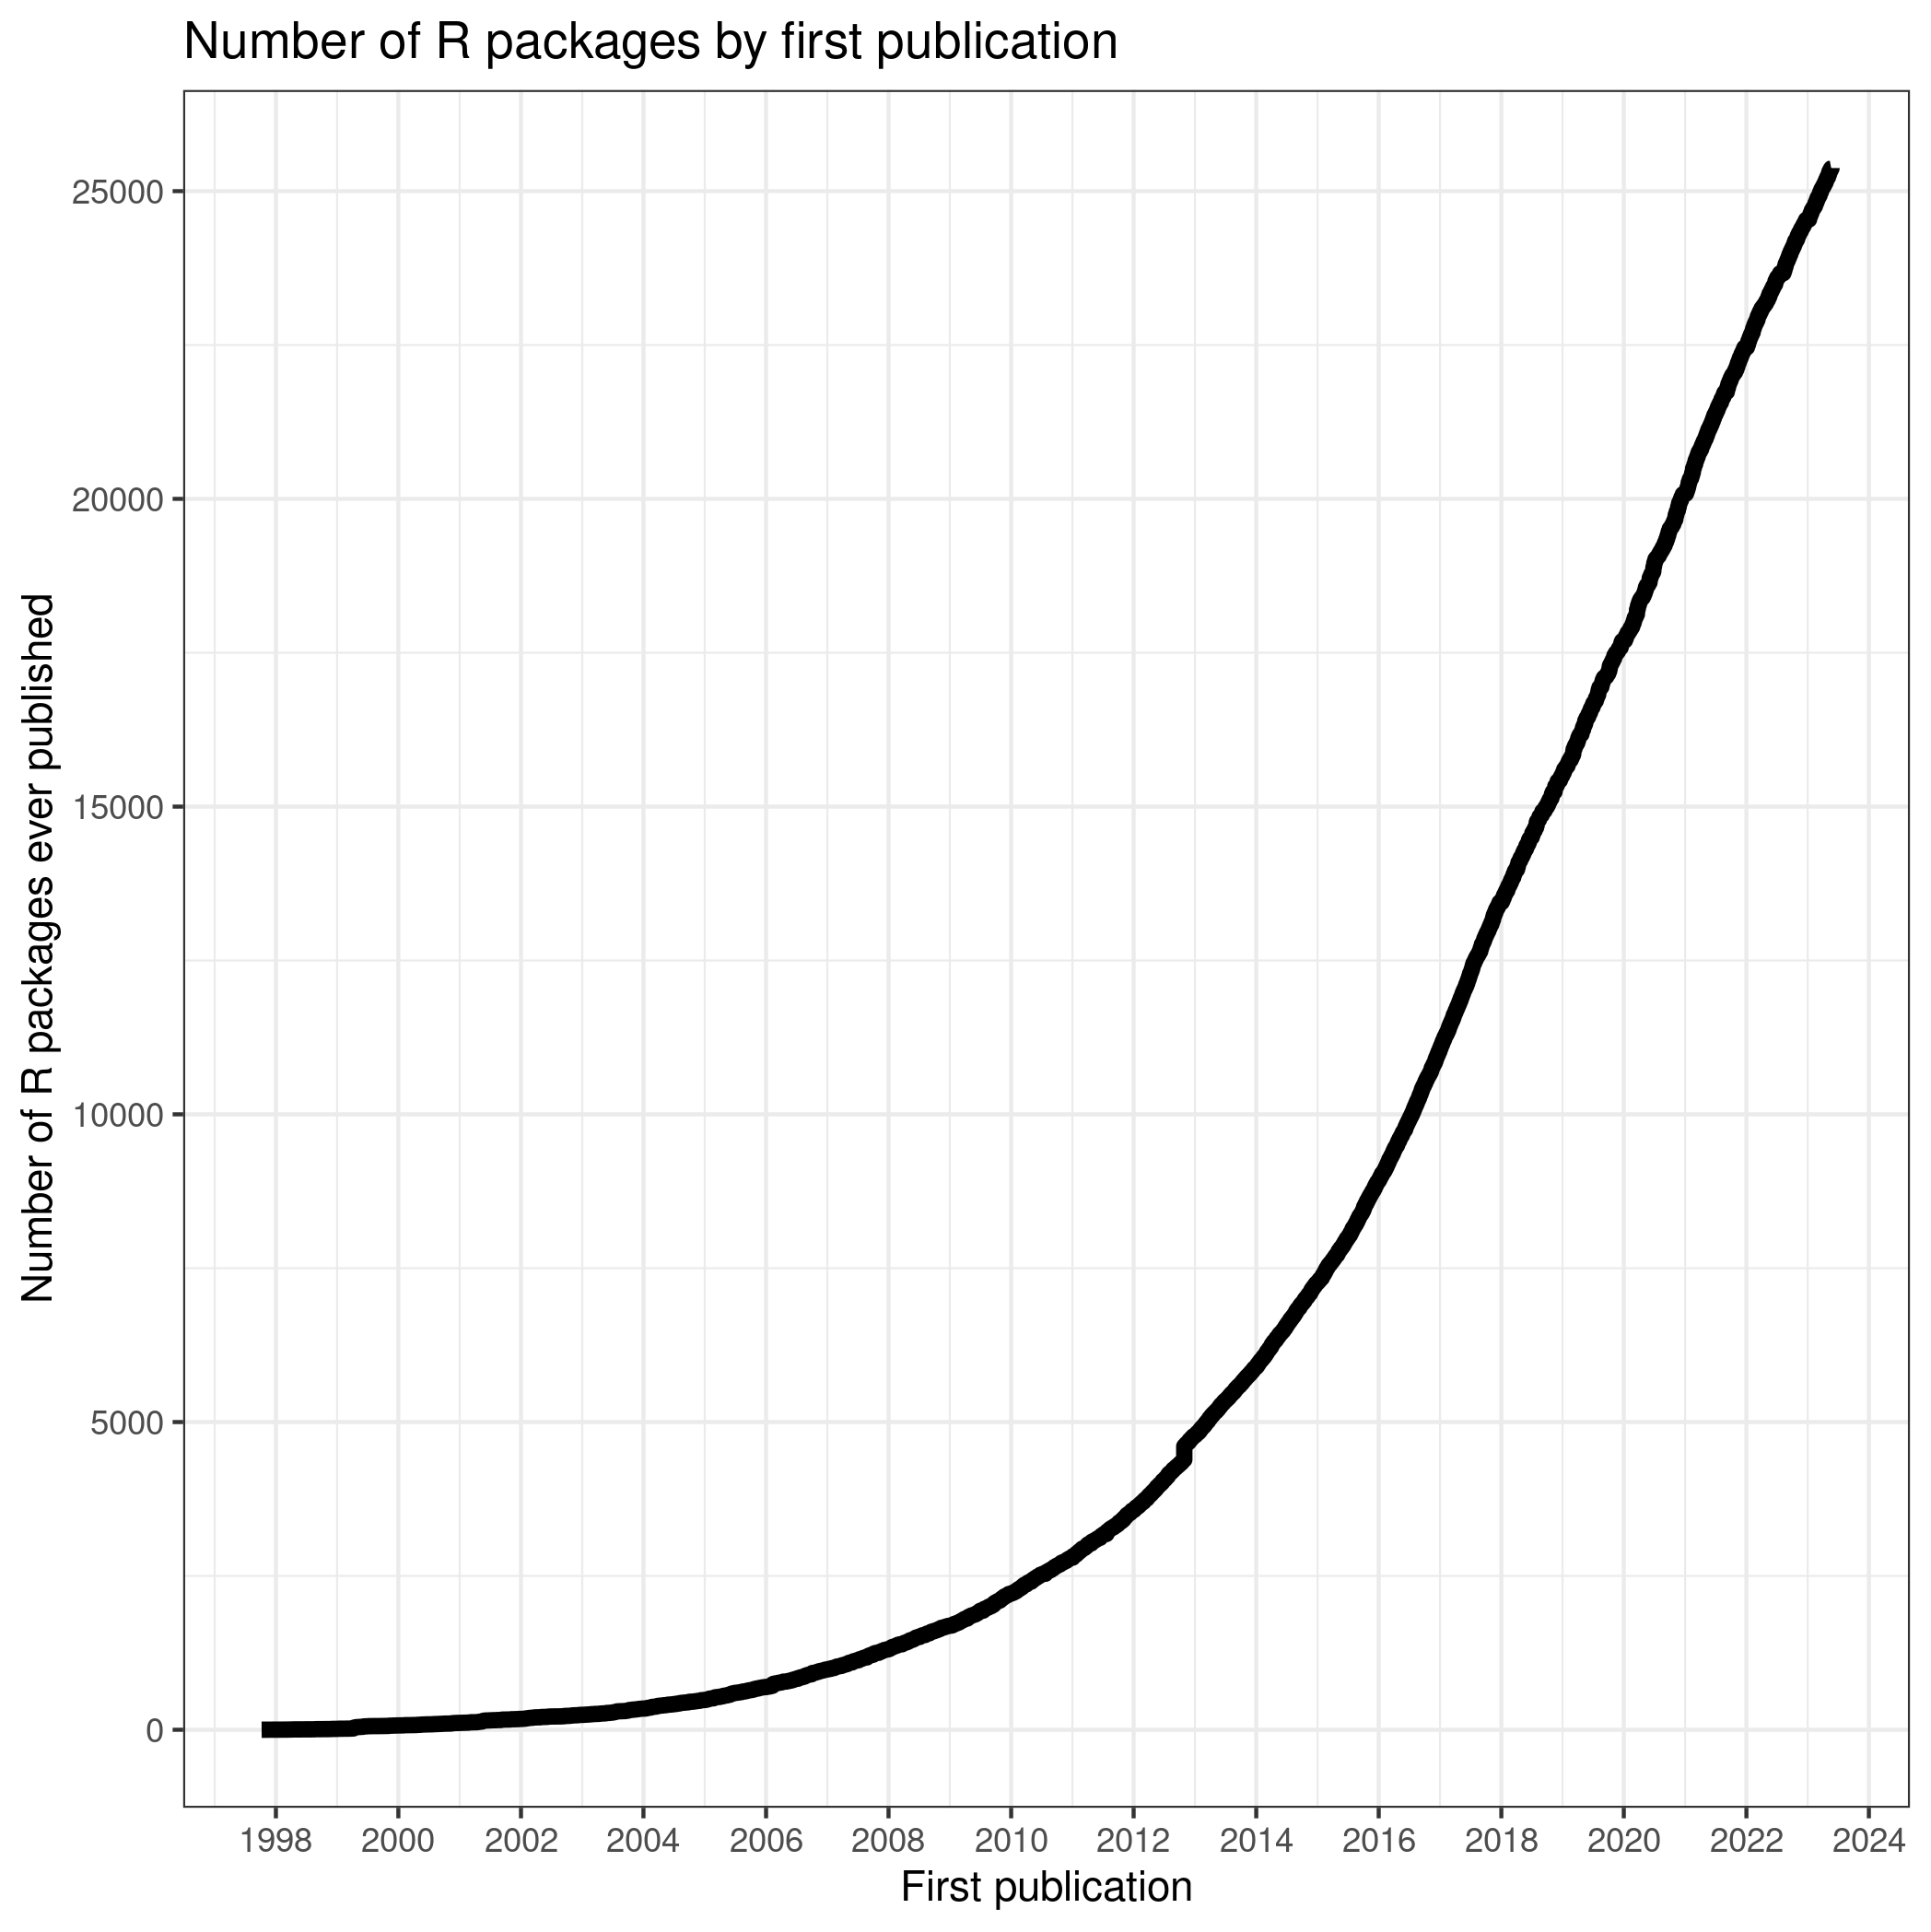
\includegraphics{figures/number-of-submitted-packages-to-CRAN.png}}

  \end{center}
  
\end{frame}

\section{Present}

\begin{frame}
  \frametitle{The present}

  The current era is characterized by
  \begin{itemize}
  \item A mature R community
  \item Large penetration of R in the commercial world (``data science'',
    ``analytics'', ``big data'')
  \item Increasing interest in the R language from computer scientists.
  \end{itemize}

\end{frame}

\begin{frame}
  \frametitle{Community}
  \begin{itemize}
  \item useR! Annual conference
    \begin{itemize}
    \item Toulouse (2019), Saint Louis (2020)
    \end{itemize}
  \item R Journal (\url{http://journal.r-project.org})
    \begin{itemize}
    \item Journal of record, peer-reviewed articles, indexed
    \item Journal of Statistical Software (JSS) has many articles
      dedicated to R packages (\url{http://jstatsoft.org})
    \end{itemize}
  \item Migration to social media
    \begin{itemize}
    \item Stack Exchange/Overflow, Github, Twitter (\#rstats)
    \item Follow @\_R\_Foundation on Twitter
    \end{itemize}
  \end{itemize}
\end{frame}

\begin{frame}
  \frametitle{Much important R infrastructure is now in package space}

  \begin{center}
  \resizebox{7cm}{!}{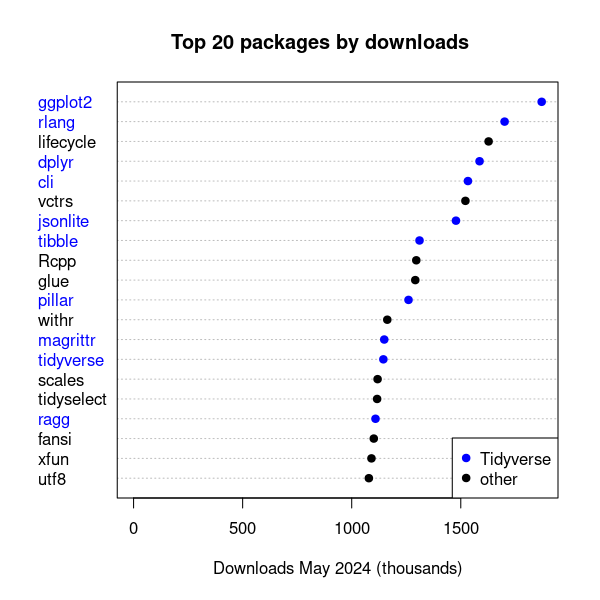
\includegraphics{figures/top20-cran.png}}
  \end{center}
    
\end{frame}

\begin{frame}
  \frametitle{Much important R infrastructure is now in package space}

  \begin{center}
  \resizebox{7cm}{!}{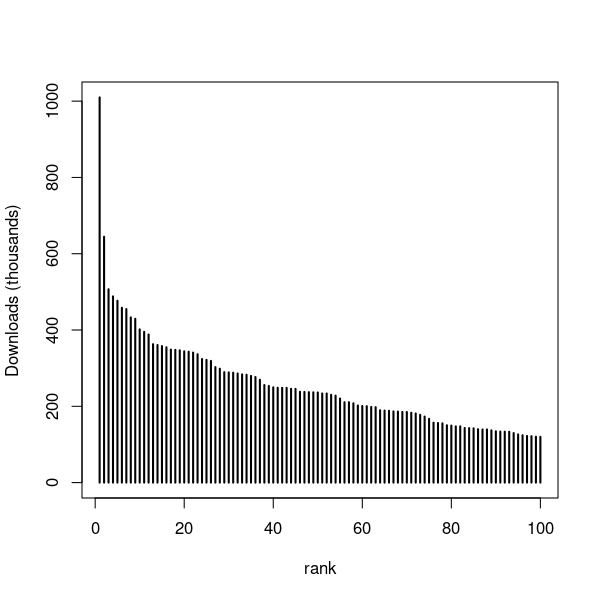
\includegraphics{figures/top100-cran.png}}
  \end{center}
    
\end{frame}

\begin{frame}[fragile]
  \frametitle{The tidyverse}
  
  \begin{itemize}
  \item Many of the popular packages on CRAN were written by Hadley Wickham
    and a team of collaborators working for the company R Studio.
  \item These packages became known as the ``hadleyverse'' until Hadley
    himself rebranded them the ``tidyverse'' (\url{www.tidyverse.org}).
  \item All packages in the tidyverse have a common design philosophy
    and work together. Common features are:
    \begin{itemize}
    \item Non-standard evaluation rules for function calls.
    \item Use of the pipe operator \verb+%>%+ to pass data
      transparently from one function call to another.
    \end{itemize}
  \item The CRAN meta-package \texttt{tidyverse} installs all of these
    packages.
  \end{itemize}
  
\end{frame}

\begin{frame}
  \frametitle{Commercial R}

  Several commercial organizations provide commercial versions of R
  including support, consulting, ...
  \begin{itemize}
  \item Revolution Computing, later Revolution Analytics (2007--2014),
    then purchased by Microsoft.
  \item RStudio (2010--)
  \item Mango Solutions (2002--)
  \end{itemize}

\end{frame}

\begin{frame}
  \frametitle{Validation and Reliability}
  \begin{itemize}
  \item {\em R: Regulatory Compliance and Validation Issues} guidance
    document by The R Foundation
  \item ValidR by Mango Solutions
  \item MRAN (\url{https://mran.microsoft.com/}), a time-stamped version of CRAN
    \begin{itemize}
    \item Allows analysis to be re-run with exactly the same package
      versions at a later date.
    \item Used by Microsoft R Open, Microsoft's distribution of R.
    \end{itemize}
  \end{itemize}
\end{frame}

\begin{frame}
  \frametitle{Forks and Clones of R}

  \begin{center}
  \begin{tabular}{llllcr}
    \hline
    Name & Language       & Commercial & Open   & Ongoing\\
         &                & sponsor    & source & \\
    \hline
    pqR     & C           &            & Yes    & Yes \\
    CXXR/rho  & C++       & Google     & Yes    & No\\
    ORBIT   & C           & Huawei     & Yes    & No\\
    \hline
    Renjin  & Java        & BeDataDriven & Yes  & Yes \\
    FastR   & Java        & Oracle     & Yes    & Yes \\
    Riposte & C++         & Tableau Research & Yes & No \\
    TERR    & C++         & TIBCO      & No     & Yes\\
    \hline
  \end{tabular}

  ~\\
  
  {\small A number of projects have looked improving the efficiency of
    R, either by forking the original codebase or by re-implementing
    R.}
  
  \end{center}
  
\end{frame}

\begin{frame}
  \frametitle{The R Foundation for Statistical Computing}

  A non-profit organization working in the public interest, founded
  in 2002 in order to:
  \begin{itemize}
  \item Provide support for the R project and other innovations in
    statistical computing.
  \item Provide a reference point for individuals, institutions or
    commercial enterprises that want to support or interact with the R
    development community.
  \item Hold and administer the copyright of R software and
    documentation (This never happened)
  \end{itemize}
  
\end{frame}
    
\begin{frame}
  \frametitle{The R Consortium}

  In 2015, a group of organizations created a consortium to support
  the R ecosystem.

  Current members (August 2019)
  \begin{description}
  \item [R Foundation] A statutory member of The R Consortium
  \item[Platinum members] Microsoft, Moore Foundation, RStudio
  \item[Gold members] TIBCO, Genentech
  \item[Silver members] Alteryx, DataCamp, Esri, Google, Mango
    Solutions, Oracle, ProCogia
  \end{description}
  
\end{frame}

\section{Future?}

\begin{frame}
  \frametitle{The Future}

  \begin{quote}
    ``Prediction is very difficult, especially about the future''
    -- variously attributed to Niels Bohr, Piet Hein, Yogi Bera
  \end{quote}

\end{frame}

\begin{frame}
  \frametitle{Trends}

  We cannot make predictions, but some long-term trends are very visible:
  \begin{itemize}
  \item Average age of R Core Team?
  \item Younger R developers more closely associated with industry
    than academia
  \item R Consortium provides mechanism for substantial investment in
    R infrastructure
%    \begin{quote}
%      ``R Consortium has invested more that \$650,000 USD in over 30
%      projects that impact the over 2 million R users worldwide'' -- R
%      Consortium press release 29 May 2018.
%    \end{quote}
  \end{itemize}
\end{frame}

%\begin{frame}
%  \frametitle{R language versus R implementation}
%
%  \begin{itemize}
%  \item R has no formal specification
%  \item R language is defined by its implementation (``GNU R'')
%  \item Long-term future of R may depend on formal specification of
%    the language, rather than current implementation.
%  \end{itemize}
%
%\end{frame}

%\begin{frame}[fragile]
%  \frametitle{Simply start over and build something better}
%
%  \begin{columns}
%    \begin{column}{4cm}
%      The {\tt x} in this function is randomly local or global
%\begin{verbatim}
%f = function() {
%   if (runif(1) > .5) 
%      x = 10
%   x
%}
%\end{verbatim}
%    \end{column}
%    \begin{column}{6cm}
%    ``In the light of this, I've come to the conclusion that rather
%    than ``fixing'' R, it would be better and much more productive to
%   simply start over and build something better'' -- Ross Ihaka,
%    Christian Robert's blog, September 13, 2010
%    \end{column}
%  \end{columns}
%
%\end{frame}

%\begin{frame}
%  \frametitle{Back to the Future}
%
%  Ross Ihaka and Duncan Temple Lang propose a new language built on
%  top of common lisp with:
%  \begin{itemize}
%  \item Scalar types
%  \item Type hinting
%  \item Call-by-reference semantics
%  \item Use of multi-cores and parallelism
%  \item More strict license to protect work donated to the commons
%  \end{itemize}
%
%\end{frame}
    
%\begin{frame}
%  \frametitle{Julia (\url{www.julialang.org})}
%
%  \begin{quote}
%    ``In Julia, I can build a package that achieves good performance
%    without the need to interface to code written in C, C++ or Fortran --
%    in the sense that my package doesn't need to require compilation of
%    code outside that provided by the language itself.
%
%    ~\\
%    
%    It is not surprising that the design of R is starting to show its
%    age. Although R has only been around for 15-18 years, its syntax
%    and much of the semantics are based on the design of ``S3'' which
%    is 25--30 years old''
%
%    ~\\
%    
%    -- Doug Bates, message to {\em R-SIG-mixed-models} list,\\
%    December 9 2013
%  \end{quote}
%  
%\end{frame}

\begin{frame}
  \frametitle{What does all of this mean for the course?}

  \begin{itemize}
  \item R incorporates over 40 years of ideas in statistical computing
    from multiple contributors.
  \item There is usually more than one way to do something in R.
  \item Some of the peculiarities of the R language are there for
    historical reasons.
  \item The course does not cover some of the recent additions to the
    R ecosystem.
  \end{itemize}

\end{frame}
    
\begin{frame}
  \frametitle{Resources}

  \begin{itemize}
  \item Chambers J, Stages in the Evolution of S
  \item Becker, R, A Brief History of S
  \item Chambers R, Evolution of the S language
  \item Ihaka, R and Gentleman R, R: A language for Data Analysis and Graphics,
    {\em J Comp Graph Stat}, {\bf 5}, 299--314, 1996.
  \item Ihaka, R, R: Past and Future History, Interface 98.
  \item Ihaka, R, Temple Lang, D, Back to the Future: Lisp as a Base for a
    Statistical Computing System
  \item Fox, J, Aspects of the Social Organization and Trajectory of
    the R Project, R Journal, Vol 1/2, 5--13, 2009.
  \end{itemize}

\end{frame}

\end{document}
